\clearpage
\section{Auswertung}
\subsection{Aufgabe 1: Bestimmung der Gitterkonstante des Sinusgitters}
In diesem Teil des Experiments bestimmten wir den Abstand der Beugungsmaxima 1. Ordnung von dem 0. Ordnung. Unsere Messungen ergaben: \[x_{links}=4,45 cm\] \[x_{rechts}=4,5 cm\] mit einem Fehler von $s_{x}=s_{x_{links}}=s_{x_{rechts}}=0,2 cm$. Die Messungenauigkeit kam dadurch zustande, dass die Punkte eine räumliche Ausdehnung hatten und die exakte Position ihrer Mitte schwer zu bestimmen war. Dies erklärt auch den kleinen Unterschied der beiden Werte, welche jedoch - wie erwartet - im Rahmen der Messungenauigkeit übereinstimmen. Um ein möglichst genaues Ergebnis zu erhalten, berechneten wir den Mittelwert zu \[\bar{x}=\frac{x_{links}+x_{rechts}}{2}=4,475 cm.\] Der Fehler berechnete sich zu \[s_{\bar{x}}=\frac{1}{2}\cdot\sqrt{(s_{x_{links}}^{2}+s_{x_{rechts}}^{2})}=\frac{s_{x}}{\sqrt{2}}=0,14 cm\] Den Abstand zwischen Gitter und Schirm vermaßen wir zu $a=(5,6\pm0,2)cm$. Mit der bekannten Formel \[\sin(\theta)=\frac{m\lambda}{K},\] der Beziehung \[\sin(\theta)=\frac{\bar{x}}{\sqrt{\bar{x}^{2}+a^{2}}}\] und den bekannten Größen $\lambda=632,8 nm$ und $m=1$ erhielten wir: \[K=\frac{m\lambda}{\sin(\theta)}=\frac{\lambda\cdot\sqrt{\bar{x}^{2}+a^{2}}}{\bar{x}}= 1,014\cdot 10^{-6}m.\] Der Fehler auf diese Größe berechnete sich zu \[s_{K}=\sqrt{\left(\frac{\partial K}{\partial \bar{x}}\right)^{2}\cdot s_{\bar{x}}^{2}+\left(\frac{\partial K}{\partial a}\right)^{2}\cdot s_{a}^{2}}=\frac{a\lambda s_{\bar{x}}}{\bar{x}^{2}\cdot\sqrt{\bar{x}^{2}+a^{2}}}\cdot\sqrt{a^{2}+2\bar{x}^{2}}=2,95\cdot10^{-8}m,\] 
Insgesamt erhielten wir für die Gitterkonstante des Sinusgitters also $K=(1,01\pm0,03)\cdot10^{-6}m$.
~\\
\subsection{Aufgabe 2: Gitterkonstante und Auflösungsvermögen der fünf Gitter.}
Bei der Bestimmung der Gitterkonstanten der fünf Amplitudengitter muss zuerst eine Eichung der Zeitachse vorgenommen werden. Hierfür wird ein Referenzgitter mit bekannter Gitterkonstante benutzt. Hier war dies ein Gitter mit der Gitterkonstante $K_{08534}=1.25 \cdot 10^{-4}m$. Dadurch lassen sich mit den bekannten Zusammenhängen die Werte von $\sin \theta $ zu den verschiedenen Ordnungen $m$ berechnen. Dazu trägt man eben diese $\sin \theta$ gegen die von uns gemessenen Zeitwerte auf. Aus dem so entstehenden linearen Zusammenhang $\sin \theta = at + b$ werden durch eine Geradenanpasssung die Werte für $a$ und $b$ bestimmt.
\newpage
\begin{figure}[h]
\begin{center}
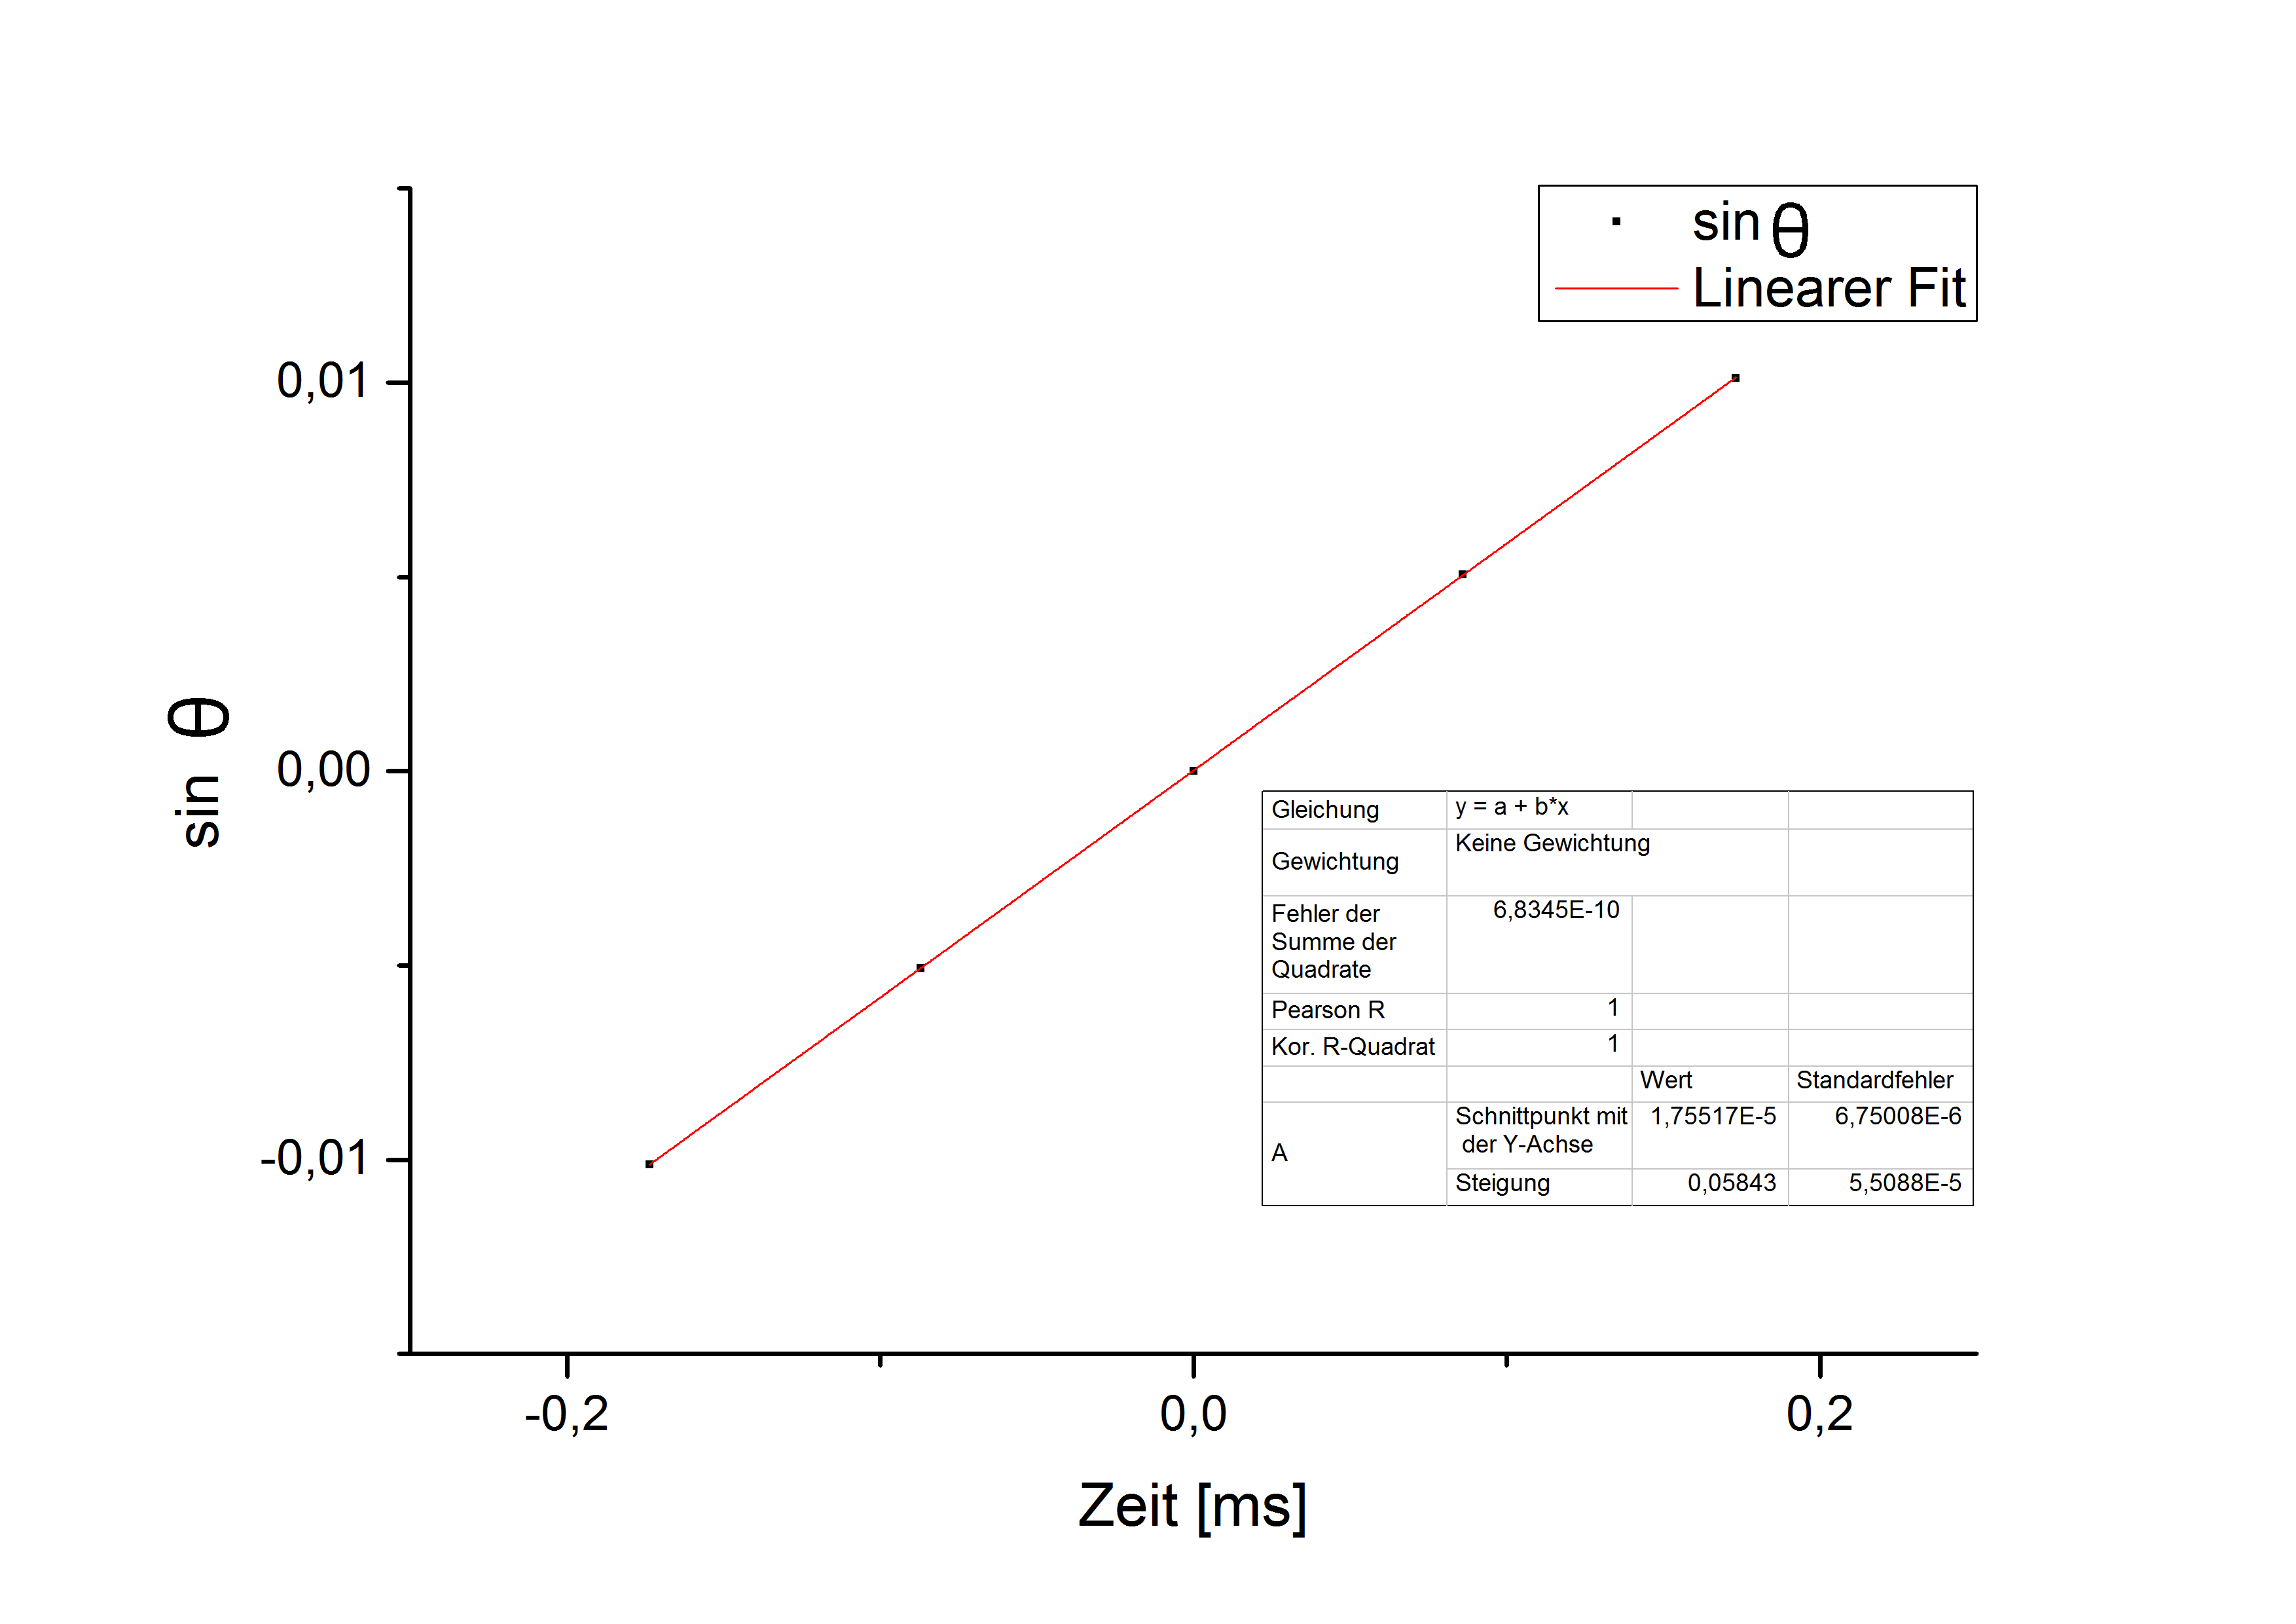
\includegraphics[scale=0.5]{lin_ref}
\caption{Eichung der Zeitachse.}
\label{fig:lin_ref}
\end{center}
\end{figure}
\noindent
Aus diesem Fit erhalten wir somit die Werte:\\
$a=(58.43 \pm 0.05) \frac{1}{s}$,\\
$b=(1.8 \pm 0.7)\cdot 10^{-5}$.\\
Mit diesen Werten können nun die Gitterkonstanten der fünf Gitter bestimmt werden. Aus den theoretischen Grundlagen folgt
\[ K=\frac{m \lambda}{at+b}\]
mit einem Fehler
\[ s_K= \sqrt{\left( \frac{\partial K}{\partial a} \cdot s_a \right)^2+\left( \frac{\partial K}{\partial b} \cdot s_b \right)^2+\left( \frac{\partial K}{\partial t} \cdot s_t \right)^2 ~} \]
\[ = \left| \frac{m \lambda}{(at+b)^2} \right| \sqrt{(a\cdot s_t)^2+(t \cdot s_a)^2 + s_b^2~} \]
Mit unseren Messungen bekommen wir nun $2m$ Werte für $K$. Aus diesen wurde das gewichtete Mittel berechnet, dadurch erhielten wir für die Gitterkonstanten $K_i$ die Werte:
\begin{center}
\begin{tabular}{ll}
Gitter 1: & $K_1=(127 \pm 1)\mu m$\\
Gitter 2: & $K_2=(33.8 \pm 0.7) \mu m$\\
Gitter 3: & $K_3=(101.2 \pm 1.5) \mu m$\\
Gitter 4: & $K_4=(101.2 \pm 1.5) \mu m$\\
Gitter 5: & $K_5=(50.8 \pm 0.9) \mu m$.\\
\end{tabular}
\end{center}
Zur Überprüfung wurde noch das zweite Referenzgitter mit bekannter Gitterkonstante $K_{08540}=100 \mu m$ vermessen. Bei diesem erhielten wir eine durch die Messung berechnete Gitterkonstante von
$K_{08540,M}=(100 \pm 37) \mu m.$\\ ~\\
Mit den oben bestimmten Gitterkonstanten wird jetzt noch das Auflösungsvermögen der Gitter bestimmt. Hierbei gilt:
\[ a=Nm=\frac{d}{K}m ~,~~~~~~~~~ mit ~ N=\frac{d}{K} \]
\[ s_a=a \cdot \sqrt{ \left( \frac{s_K^2}{K^2} \right)^2 + \left( \frac{s_d^2}{d^2} \right)^2 ~ } \]
Wie man im Anhang sehen kann beträgt der Durchmesser des Strahls $d=(3.5 \pm 0.5)mm$. $m$ steht hier für die höchste sichtbare Ordnung.\\
Somit erhält man folgende Auflösungsvermögen:\\
\begin{center}
\begin{tabular}{ll}
Gitter 1: & $a_1=137 \pm 20$\\
Gitter 2: & $a_2=104 \pm 15$\\
Gitter 3: & $a_3=173 \pm 25$\\
Gitter 4: & $a_4=173 \pm 25$\\
Gitter 5: & $a_5=138 \pm 20$\\
\end{tabular}
\end{center} ~\\
\subsection{Aufgabe 3: Berechnung der Aperturfunktion aus den ermittelten Intensitäten}
Zur Berechnung der Aperturfunktion wird wie beschreiben die Fourierreihe als Näherung benutzt
\[ g(x)=\sum\limits_{j=0}^{\infty}\pm\sqrt{I_{j}}\cdot\cos\left(\frac{x}{K}\cdot 2\pi j\right). \]
Mit den Werten für die Intensitäten der einzelnen Maxima kann diese approximiert werden.
\[ I_0=1.60788 V \]
\[ I_1=8.3115 \cdot 10^{-2} V \]
\[ I_2=5.9515 \cdot 10^{-2} V \]
\[ I_3=3.79125 \cdot 10^{-2} V \]
\[ I_4=1.3515 \cdot 10^{-2} V \]
\[ I_5=7.515 \cdot 10^{-3} V \]
Bei den Intensitäten welche doppelt vorhanden sind wurde der Mittelwert berechnet. Der Fehler aus den Mittelwerten berechnet sich aus $s_I=\frac{s_{I_{mess}}}{\sqrt{2}}$, wobei $s_{I_{mess}}$ der Fehler der Einzelmessung ist.\\
Hieraus ergibt sich somit folgendes Diagramm:
\begin{figure}[h]
\begin{center}
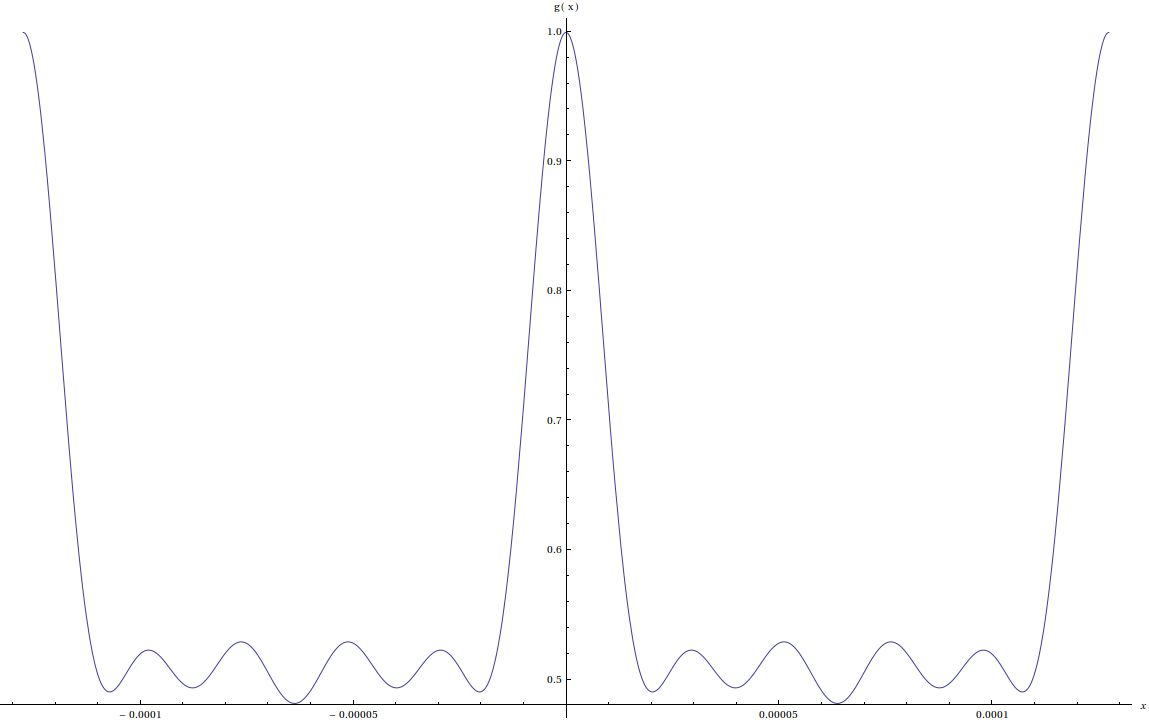
\includegraphics[scale=0.35]{aperturfunktion}
\caption{Zwei Perioden unserer approximierten Aperturfunktion.}
\label{fig:aperturfunktion}
\end{center}
\end{figure}
\clearpage
\subsection{Aufgabe 4: Verhältnis der Spaltbreite zur Gitterkonstante}
Aus der oben bestimmten Aperturfunktion kann nun das Verhältnis der Spaltbreite zur Gitterkonstante bestimmt werden. Dazu wir die Spaltbreite $w$ aus der Breite des halben Maximums der Aperturfunktion numerisch bestimmt. Den Spaltabstand $d$ erhält man mit der Gitterkonstante durch $d=K-w$. Somit lässt sich das Verhältnis $v=\frac{w}{d}$ berechnen, wobei hier für den Fehler $s_v = v \frac{s_d}{d}$ gilt. Somit erhalten wir ein Verhältnis von:
\[ v= ** \pm ** .\]